% Training curves, baseline (matched protocol) and extension on shared axes. Drawn for this work by
%   ../tse_venv/bin/python scripts/plot_training_curves.py --layout terms-wer --out report/figures/training_curves.pdf
% from both runs' history.csv and every matching live-judge run
% (sir0_val, both, n=103). Baseline = 2026-10-07-train-sir0-baseline-matched-s1, session 1
% of 2 (epochs 0-13); session 2 and its judge runs appear on re-running the command above
% once they exist. The original 16-epoch baseline run (2026-09-04) is no longer drawn.
\begin{figure}[htbp]
  \centering
  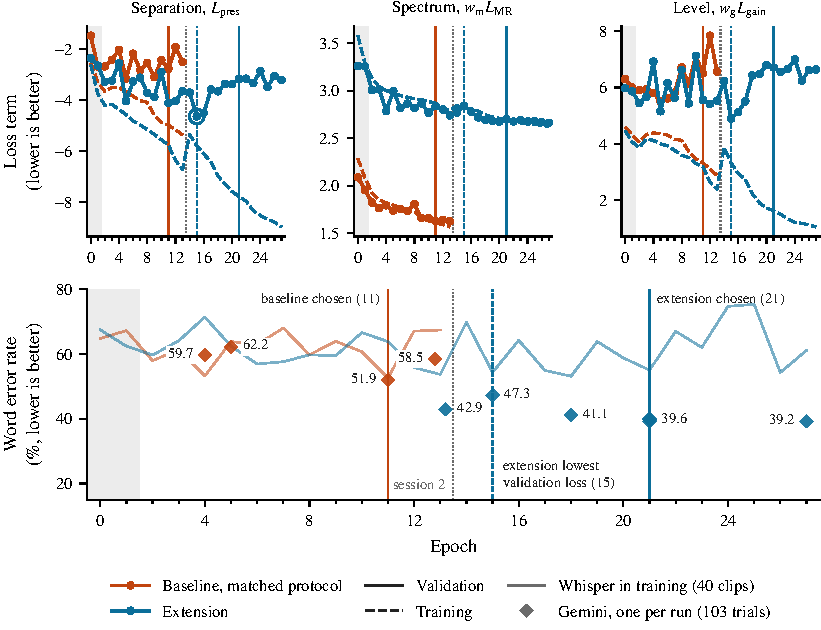
\includegraphics[width=\textwidth]{figures/training_curves.pdf}
  \caption{Training (dashed) and validation (solid) scores per epoch, counted from zero, for the baseline (orange) and the extension (blue), trained under the same protocol: the in-training Whisper check sets the learning rate and decides which epochs are kept. The baseline shown is epochs 0--13 of a 28-epoch run and is not yet judged; it is not the earlier baseline run that gives epoch 6 in the results tables. Top: the three weighted terms of the target-present loss, the first bracket of \autoref{eq:total}, which add up to it (lower is better): separation $L_\textup{pres}$, spectrum $w_\textup{m} L_\textup{MR}$ and level $w_\textup{g} L_\textup{gain}$. Bottom: word error rate on the 103 validation trials with both speakers present (lower is better). Each diamond is one run of the live judge on the same audio, labelled with the mean of the runs at that epoch; the thin lines are the in-training Whisper \texttt{small.en} check on 40 validation clips. Shaded epochs fail the \SI{-10}{dB} silence bar in both runs. The solid vertical line marks the extension's chosen epoch, the dashed one its lowest validation loss (the sum of the three terms), and the grey dotted line where training resumed in a second session.}
  \label{fig:training_curves}
\end{figure}
